\input{preamble.tex}

\usetikzlibrary {datavisualization}

\newcommand{\tableaucroise}[4]{
\begin{tabular}{|c|c|c|c|}
	\cline{2-4}
	\multicolumn{1}{c|}{} & #1 \\ \hline
	#2 \\ \hline
	#3  \\ \hline
	#4  \\ \hline
\end{tabular}
}

\begin{document}

\reversemarginpar

\pagestyle{fancy}
\fancyhead[L]{Terminale STMG}
\fancyhead[C]{\textbf{DS n°7c : probabilités conditionnelles}}
\fancyhead[R]{\today}

\null\vspace{-30pt}
Nom / Prénom : \\

Consignes particulières : 
\begin{itemize}[label=$\bullet$]
	\item 
	La calculatrice est {autorisée}.
	\item 
	Les exercices \ref{exe:1} et \ref{exe:2} peuvent être faits partiellement sur la feuille.
	\item 
	Toute trace de recherche est prise en compte.
\end{itemize}

\hrule

\exe{5}{
On considère deux évènements $A$ et $B$ et on donne :
\begin{multicols}{2}
\begin{enumerate}[label=(\roman*)]
\item $P_{\widebar{B}}(A) = 0,65$
\item $P_B(A) = 0,4$
\item $P(\widebar{B}) = 0,7$
\end{enumerate}
\end{multicols}
\begin{enumerate}
\item
Compléter l'arbre ci-dessous :
\begin{center}
\begin{tikzpicture}[scale=1]
\node {}[grow=right, level distance=4cm, sibling distance=2cm]
	child {node {\small $\widebar{B}$}[level distance=4cm, sibling distance=1cm]
		child {node{\small $\widebar{A}$}			
		}
		child {node{\small $A$}
		}
	}
	child {node {\small $B$}[level distance=4cm, sibling distance=1cm]
		child {node{\small $\widebar{A}$}
		}
		child {node{\small $A$}
		}
	}
;
\end{tikzpicture}
\end{center}
\begin{multicols}{2}
\item Calculer $P(A \cap B)$.
\item Calculer $P(A \cap \overline{B})$.
\item  Calculer $P(A)$.
\item Calculer $P_A(B)$.
\end{multicols}
\end{enumerate}
}{exe:1}{
\begin{enumerate}
\item
\begin{center}
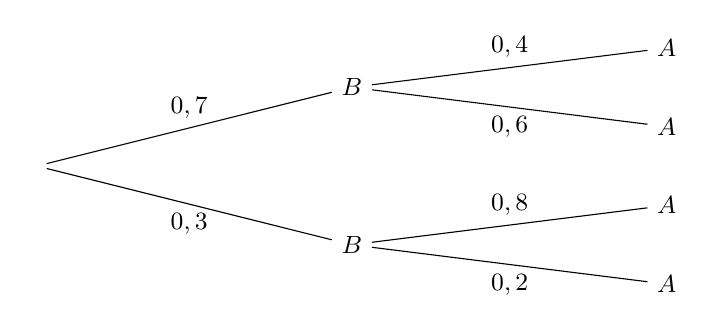
\begin{tikzpicture}[scale=1]
\node {}[grow=right, level distance=4cm, sibling distance=2cm]
	child {node {\small $\widebar{B}$}[level distance=4cm, sibling distance=1cm]
		child {node{\small $\widebar{A}$}
			edge from parent node[below] {\small $0,2$}				
		}
		child {node{\small $A$}
			edge from parent node[above] {\small $0,8$}	
		}
		edge from parent node[below] {\small $0,3$}	
	}
	child {node {\small $B$}[level distance=4cm, sibling distance=1cm]
		child {node{\small $\widebar{A}$}
			edge from parent node[below] {\small $0,6$}	
		}
		child {node{\small $A$}
			edge from parent node[above] {\small $0,4$}
		}
		edge from parent node[above] {\small $0,7$}	
	}
;
\end{tikzpicture}
\end{center}
\begin{multicols}{2}
\item $P(A \cap B) = 0,7 \times 0,4 = 0,28$.
\item $P(\overline{A} \cap \overline{B}) = 0,3 \times 0,2 = 0,06$.
\item $P(A) = 0,7 \times 0,4 + 0,3 \times 0,8 = 0,52$.
\item $P_A(B) = \dfrac{P(B)}{P(A)} P_B(A) = \dfrac{0,7}{0,52} \times 0,4 \approx 0,54$.
\end{multicols}
\end{enumerate}
}

\exe{5}{
Un assureur souhaite ajuster le tarif de ses contrats. Il fait un sondage de ses 2~350 véhicules assurés. 
Parmi ces derniers, 1~500 sont des véhicules de tourisme, le reste sont des utilitaires.
Parmi les véhicules de tourisme, 150 ont été impliqués dans des accidents durant l'année.
Parmi les véhicules utilitaires, 95 ont été impliqués dans des accidents.
\begin{enumerate}
\item Compléter le tableau croisé d'effectifs ci-dessous :
	\begin{center}
	%\def\arraystretch{1.8}
	\setlength\tabcolsep{20pt}
	\tableaucroise{Tourisme & Utilitaire & Total}{Accident & & &}{Sans accident & & &}{Total &&&}
	\end{center}
\item On considère que ces données sont représentatives de tout le parc automobile assuré. Calculer :
\begin{enumerate}
\item la probabilité qu'un véhicule soit impliqué dans un accident ;
\item la probabilité qu'un véhicule soit impliqué dans un accident sachant que c'est un utilitaire ;
\item la probabilité qu'un véhicule \textbf{ne soit pas} impliqué dans un accident sachant que c'est un utilitaire ;
\end{enumerate}
\item Les évènements \og le véhicule est impliqué dans un accident \fg{} et \og le véhicule est un utilitaire \fg{} sont-ils indépendants ?
Justifier.
\end{enumerate}
}{exe:2}{

}

\exe{5}{
On lance deux fois de suite une pièce dont on ne connait pas la probabilité de tomber sur pile.
On note $P$ et $F$ les évènements suivants :
\begin{enumerate}[label=(\roman*)]
\item P : \og la pièce tombe sur pile \fg{};
\item F : \og la pièce tombe sur face \fg.
\end{enumerate}
et on note $p$ la probabilité de l'évènement $P$.
\begin{enumerate} 
\item Construire l'arbre pondéré représentant cette situation.
\item Montrer que la probabilité d'obtenir deux fois de suite pile est égale à $p^2$.
\item On consate que la probabilité d'obtenir deux fois de suite pile est égale à $0,16$. 
\begin{enumerate}
\item En déduire la valeur de $p$.
\item Calculer la probabilité d'obtenir deux fois de suite face.
\item Calculer la probabilité d'obtenir une fois face et une fois pile (peu importe l'ordre).
\end{enumerate}
\end{enumerate}
}{exe:3}{

}

\exe{5}{
Un météorologiste amateur a établi une méthode pour prévoir s'il va pleuvoir. Il note $Pl$ et $N$ les deux évènements suivants :
\begin{enumerate}[label=(\roman*)]
\item
$N$ : \og le ciel est nuageux \fg. 
\item
$Pl$ : \og il pleut \fg. 
\end{enumerate}
Le météorologiste observe que la probabilité que le ciel soit nuageux sachant qu'il pleut est de 99 \% . \\
Il observe aussi que la probabilité que le ciel soit nuageux sachant qu'il ne pleut pas est de 40 \% .
\begin{enumerate}
\item Sur dix années (3~652 jours d'obsevation), le météorologiste a observé 548 jours de pluie. 
Proposer une estimation de $P(Pl)$.
\item Représenter la situation par un arbre de probabilité.
\item Calculer la probabilité que le ciel soit nuageux.
\item Calculer la probabilité qu'il pleuve sachant que le ciel est nuageux.
\item Commenter sur la méthode du météorologiste.
\end{enumerate}
}{exe:4}{

}



%%%%%%%%%%%%%

%\newpage
%\fancyhead[C]{\textbf{Solutions}}
%\shipoutAnswer


\end{document}
